% !TEX root = ../ac_paper.tex

\section{Language Modeling}

In this section, we discuss a model for the ``language" of balanced presentations. Each presentation with two relators is a string of six letters, better called "tokens" in the nomenclature of Natural Language Processing, i.e. $x$, $y$, $x^{-1}$, and $y^{-1}$, and two ``stop tokens" --- one that separates two relators of a presentation, and another that marks the end of a presentation. Given this vocabulary $V$ of six tokens, we can ask what is the probability $p(t_1, \cdots, t_N)$ for $t_i \in V$ of the occurence of a specific presentation in the space of all balanced presentations. Using the chain rule of probability theory, 
\[
p(t_1 \cdots t_{N}) = \prod\limits_{i=1}^{N} p (t_{i} \mid t_{1} \cdots t_{i-1}) 
\]

Here $p (t_{n} \mid t_{1} \cdots t_{n-1})$, often called the $n$-gram probability distribution, is the probability of a token $t_n$ following a sequence of tokens $t_{1} \cdots t_{n-1}$. In order to model the language of balanced presentations, we would like to estimate the $n$-gram probability distributions. 

Over the last few years, Transformer models have shown great success in modeling human-understandable languages to the extent that these models can write text almost indistinguishable from human-written texts. Specifically, the architecture used for modeling language is the auto-regressive "decoder-only" Transformer, which we review in detail in section 5.1. In section 5.2, we discuss the method with which we generate the dataset required for training the model. Finally, in section 5.3, we provide details of some insights we learned from this process. 

\subsection{Transformers: a review}

Here, we give a short review of the architecture of a decoder-only transformer. For more detailed descriptions, see \cite{elhage2021mathematical, vaswani2023attention, douglas2023large}. 


Previously, encoder-only architectures were used in  for the unknot decision problem. 

Given an input sequence $t_1, t_2, \cdots, t_{N}$, a decoder-only transformer predicts the probability distribution $p(t \mid t_1, t_2, \cdots, t_{N})$ over the set $V$ of tokens of size $n_{\text{vocab}}$. The probability is computed by applying the softmax function to the logits $T(t)$, which are estimated by applying the following sequence of operations.

First, assign to each token in the vocabulary a distinct label in the range $1, 2, \cdots, n_{\text{vocab}}$; re-writing the original sequence as a sequence of integers, which we also label as $t_i$. Next, write the sequence in terms of "one-hot encoded vectors", i.e. a matrix $t  \in \R^{N \times n_{\text{vocab}}}$ such that 
\[
t_{ij} = \delta_{i t_i}
\]
and embed the sequence in a $\dm$-dimensional vector space, 
\[
x_0 = (W_P \otimes W_E) t
\]
Here, $W_P \in \R^{\dm \times N}$ and $W_E \in \R^{\dm \times n_{\text{vocab}} }$ are positional and token embedding matrices, which are learned by gradient descent. 
\footnote{Note that $t$ and all $x_j$ are two-dimensional tensors, so it is appropriate to apply tensors of linear transformations to them. Often in a transformer architecture, these operations are of the form $\mathbb{1} \otimes \cdots$; in these cases, we write the operation simply as $\cdots$, dropping the tensor product with the identity transformation. For example, $\mathbb{1} \otimes W_U$, $\mathbb{1} \otimes W^m_I$, $\mathbb{1} \otimes W^m_O$, etc. are all often simply written as $W_U$, $W^m_I$, $W^m_O$. It is clear from the dimensionality of these matrices that they act as $\mathbb{1} \otimes \cdot$.}
An $L$-layer transformer alternates between applying a ``multi-head attention layer" ($\sum\limits_{h \in H} h$) and an ``MLP-layer" ($m$) $L$ times. For $i=0, \cdots, L-1$,
\[
\begin{aligned}
x_{2i+1} &= x_{2i} + \sum_{h \in H} h(\LN(x_{2i})), \\
x_{2i + 2} &= x_{2i + 1} + m(\LN(x_{2i + 1})).
\end{aligned}
\]
Each $x_j$ is a matrix in $\mathbb{R^{N \times \dm}}$, with the interpretation that its $i$-th row is the embedding of the sequence $t_1, \cdots, t_i$ in the $\dm$-dimensional embedding space as learned by the preceeding $j$ operations. Finally, one applies an "unembedding layer" to convert $\dm$-dimensional vectors to $n_{\text{vocab}}$-dimensional vector of "logits" $T(t)$ that estimate the sought-after probability distribution,
\[
\begin{aligned}
T(t) &= W_U x_{2L-1} \\
p(t) &=\softmax (T(t))
\end{aligned}
\]

The functions $\LN$, $m$ and $h$ are defined as follows. $\LN$ is the "Layer-Norm" operation intended to normalize the input of each layer to make the optimization process more feasible,
\[
LN(x) = \left(\mathbb{1} \otimes \text{diag}(\gamma) \right) \frac{(x-\overline{x})}{\sqrt{\text{var}(x)}} + \mathbb{1} \otimes \beta
\]
Here, $\gamma, \beta \in \mathbb{R}^{\dm}$ are learnable parameters. $\overline{x}$ and $\text{var}(x)$ are mean and variance of each row of $x$.

The MLP-layer $m$ is a non-linear operation, 
\[
m(x) =W^m_O \ \text{max}(W_I^m x, 0)
\]
with learnable parameters $W^m_I \in \mathbb{R}^{d_{\text{MLP}} \times \dm}$, $W^m_O \in \mathbb{R}^{\dm \times d_{\text{MLP}}}$. It is standard to take $d_{\text{MLP}} = 4 \dm$.

Finally, the multi-headed attention-layer $\sum_{h \in H} h$ is a sum of $n_{\text{heads}}$ ``attention-head" operations $h$, 
\[
h(x) = (A^h(x) \otimes W^h_O W^h_V) x
\]
where $W^h_V \in \R^{d_{\text{head}} \times \dm}$, 
$W^h_O \in \R^{\dm \times d_{\text{head}}}$ 
are matrices of learnable parameters. 
$d_{\text{head}}$ is the "attention-head dimension" that satisfies $d_{\text{head}} \times n_{\text{head}} = d_{\text{model}}$. 
The attention matrix $A^h$ is computed with the help of learnable matrices 
$W^h_Q, W^h_K \in \R^{d_{\text{head}} \times \dm}$,
\[
A^h(x) = \softmax^\star \left(\frac{x^T (W^h_Q)^T W^h_K x}{\sqrt{d_{\text{head}}}}\right)
\] 
The attention-head is an $N \times N$ matrix. The element $A^h(x)_{ij}$ 
is interpreted as the "attention" paid to the token 
$t_j$ in estimating 
$p(t_{i+1} \mid t_1, \cdots, t_i)$. $\softmax^\star$
is a variant of the $\softmax$ function suitable for auto-regressive tasks: it sets all the elements in the upper triangle of its input before applying the 
$\softmax$ operation. 
That is, future tokens --- $t_k$ for $k > i$, play no role in the prediction of $p(t_{i+1} \mid t_1, \cdots, t_i)$.

We train the transformer model by minimizing the cross-entropy loss between the estimated and the true probability distributions of $p(t_{i+1} | t_1, \cdots, t_{i})$ for all $i$. This offers parallelism, which is useful for efficient training of our models. 

Before we discuss the dataset we used to train our model, we present an important remark. In practice, the embedding matrix $W_E$ and the unembedding matrix $W_U$ are often "tied" together, i.e. $W_E = W_U^T$. The rows of $W_E = W_U^T$ are interpreted as the embeddings of words/sentences, to which one can apply the usual operations of a vector space to gain insights \cite{Bengio:2003}. For example, the cosine of the angle between two embedding vectors, also known as "cosine similarity", is often used to measure the similarity between two texts. \fixme{add a citation here.}\footnote{\fixme{What is the correct reference for analyzing embeddings through cosine simiarity between vectors?}}


\subsection{Dataset for the GPT model}

In this section, we discuss the training and validation datasets we used to train and evaluate our Transformer models. 

We apply sequences of AC moves to the Miller-Schupp series presentations studied in the previous subsection to generate a dataset.
We use Algorithm \autoref{alg:apply_ac_moves} to ensure that the total length of the generated presentations follows roughly a uniform distribution.
(See \autoref{fig:gpt_data}; there, the distribution is roughly uniform with short tails on either side.)
\footnote{Maybe there should be only one histogram in the figure showing combined solved+unsolved statistics.
As it is, I computed separate percentages for each solved/unsolved case.
I should clarify that if I leave the figure as it is.
It is also good to change the total length.
Also change the label of x-axis to something better.}

Algorithm \autoref{alg:apply_ac_moves} generates presentations of increasing lengths in $n$ phases.
In the $i$-th phase, presentations with maximum relator length $l_i$ are generated, where $l_i$ is sampled from a discrete uniform distribution with bounds $l + i l_{\text{inc}} $ and $l + (i+1) l_{\text{inc}}$.
Here, $l$ is the maximum of the lengths of the two relators in the initial Miller-Schupp presentation $R_0$ (and thus the minimum value of maximum relator length in the algorithm), and $l_{\text{inc}}$ is defined in terms of the maximum possible relator length $l_{\text{max}}$ we wish to obtain in the last phase as $l_{\text{inc}} = (l_{\text{max}}-l)/n$.
In the $i$-th phase, $T$ AC moves are applied to a presentation generated in the $(i-1)$-th phase.
In our work, we chose $l_{\text{max}}=128$, $n=128$, $m=12$, and $T=1000$.
\footnote{Specify much earlier in the paper, and here as well, that whenever we apply AC moves, we set a maximum length up to which each relator is allowed to grow.
Any AC move that would result in a presentation of longer relator length acts trivially.
Maybe instead of writing $A \sim \text{AC Moves}$, there should be a notation like $(AC)_l$ when $l$ is specified to be the maximum relator length.}

\begin{algorithm}
	\caption{Generate AC Cousins}\label{alg:apply_ac_moves}
	\begin{algorithmic}
		\Require $R_0$, $l_{\text{max}}$, $n$, $m$, $T$
		\State $L \gets \{ \}$ \Comment{Initiate the list $L$ of all presentations}

		\State $l \gets \max(l_1, l_2)$

		\Comment{Set $l_1$, $l_2$ are the lengths of relators of $R_0$}

		\State $l_{\text{inc}} \gets (l_{\text{max}}-l)/n$

		\Comment{The increment by which the maximum relator length increases in each phase}

		\For {$i = 1, 2, \dots, n$}

		\Comment{Loop over $n$ phases}
		\For {$j = 1, 2, \dots, m$}

		\Comment{Generate $m$ presentations in each phase}
		\State $l_i \sim \mathcal{U}(l + i l_{\text{inc}} , l + (i+1) l_{\text{inc}})$

		\Comment{Set the maximum relator length for $i$-th phase}
		\If{i is 0}
		\State $R \gets R_0$
		\Else
		\State $R \gets L[(i-1) \times m+j]$
		\EndIf

		\Comment{Set $R$ to a presentation of the previous phase if $i > 0$, else set it to the initial presentation $R_0$}


		\For{$k = 1, 2, \dots, T$}

		\Comment{Apply $T$ randomly selected AC-moves}
		\State A $\sim$ AC Moves
		\State $R \gets A \cdot R$

		\EndFor

		\State $L \gets R$

		\Comment{Add the resultant presentation $R$ to $L$}

		\EndFor
		\EndFor
	\end{algorithmic}
\end{algorithm}

The main reason for choosing this algorithm is so that our GPT model sees roughly the same amount of presentations of each length and is, hence, not biased towards shorter or longer presentations.
The final dataset contained 0.8 million (1 million) presentations generated from applying Algorithm \autoref{alg:apply_ac_moves} to BFS-easy (BFS-hard) examples.
Only a small amount (roughly 15 percent) of the original Miller-Schupp presentations remained to be part of this dataset.

\begin{figure}
	\centering
	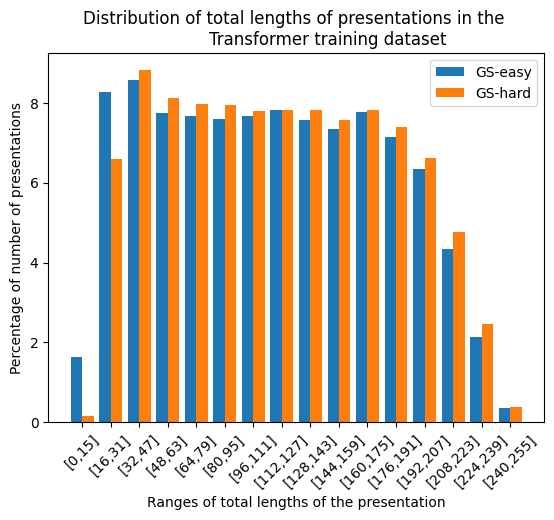
\includegraphics[scale=0.6]{fig/gpt_data_length_distribution.png}
	\caption{Percentage of presentations in various ranges of total lengths.}
	\label{fig:gpt_data}
\end{figure}

The dataset is tokenized by adding two stop tokens that represent the end of two relators of a presentation.
Thus there are six tokens in total: one each for $x$, $y$, $x^{-1}$, and $y^{-1}$ and the two stop tokens.
The tokenized dataset has about 217M tokens, and the distribution of tokens is shown in \autoref{fig:tokens_hist}.
We note that $y$ and $y^{-1}$ appear significantly more often than $x$ and $x^{-1}$ in the unsolved dataset.
This is likely because the BFS-hard examples have higher $n$, and higher $n$ corresponds to more of a presence of $y$ and $y^{-1}$.
Interestingly, this effect remains in the dataset even when we apply thousands of AC moves.
I should investigate this further.

We set aside 10 percent of the data as a validation dataset.

\begin{figure}
	\centering
	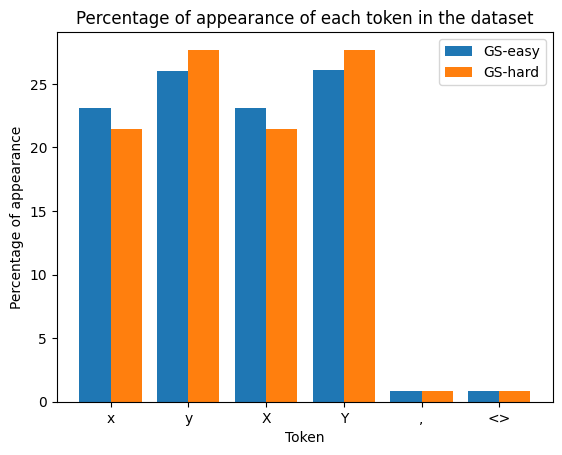
\includegraphics[scale=0.6]{fig/tokens_hist.png}
	\caption{Percentage of appearance of each token in the solved/unsolved datasets.}
	\label{fig:tokens_hist}
\end{figure}

\subsection{Results}
We train a GPT model on the dataset described in the previous subsection.
Given a context of $n$ tokens, a GPT model learns the probability distribution for $(n+1)$-st token.
The extent to which it can make good predictions is measured by a cross-entropy loss defined above.
We trained a model with embedding dimension 512 and 8 layers.
The model is initialized with random weights that assigns an equal probability to each token, thus the initial value of the cross-entropy loss is $-\ln(1/6) \sim 1.7917$.
As the model was trained, we were able to achieve the minimum validation loss of 0.5685.
\footnote{insert a validation loss curve.}

We use the trained model to obtain embeddings of the 1190 Miller Schupp presentations studied above.
To visualize these embeddings, we use t-SNE with distance measured by the cosine of the angle between two embedding vectors and project the embedding space down to two dimensions. \fixme{Try to understand how cosine similarity changes formulas for t-SNE.}  Value of perplexity? Were the results robust under the change of perplexity?
\fixme{Should we also plot UMAPs?}
The final result is shown in \autoref{fig:embeddings_tsne}.
We see that the model has clustered together examples with the same $n$.

\footnote{Maybe I should replace 'Solved' and 'Unsolved' with 'BFS-easy' and 'BFS-hard' in all the images.}

\begin{figure}
	\centering
	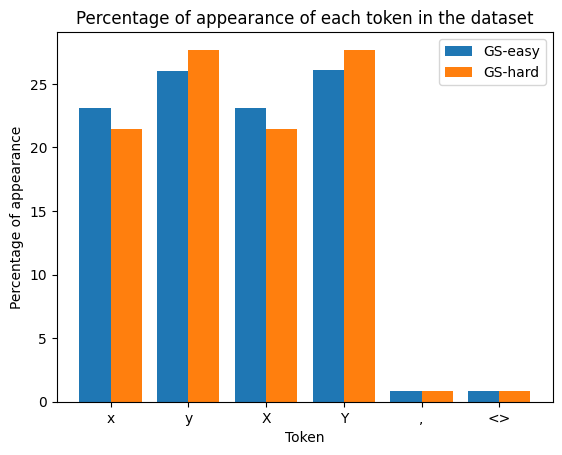
\includegraphics[scale=0.6]{fig/tokens_hist.png}
	\caption{Percentage of appearance of each token in the solved/unsolved datasets.}
	\label{fig:tokens_hist}
\end{figure}

\begin{figure}
	\centering
	\begin{subfigure}[b]{\textwidth}
		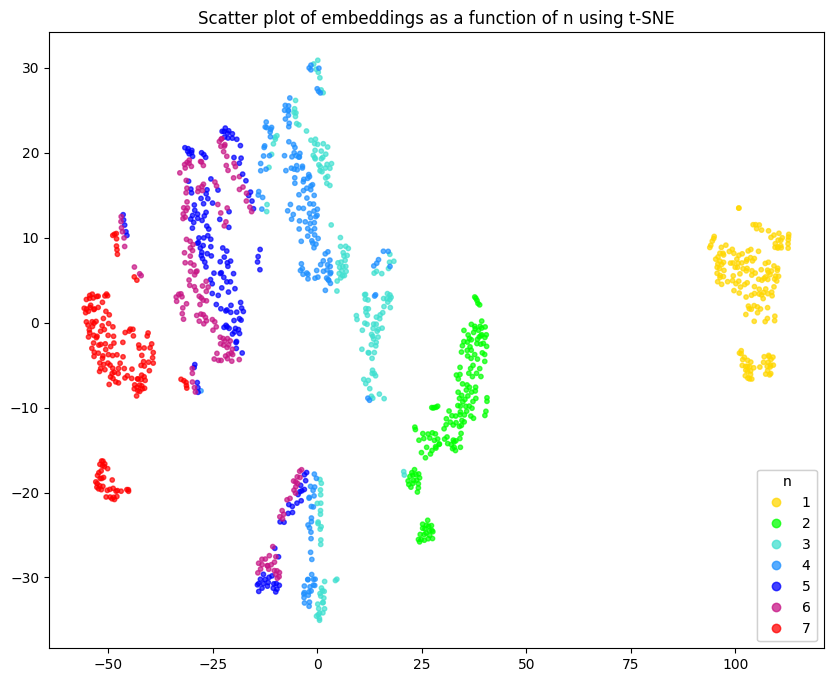
\includegraphics[width=\linewidth]{fig/embeddings_n.png}
		\caption{Scatter plot of embeddings as a function of $n$ using t-SNE}
		\label{fig:hist_vs_n}
	\end{subfigure}%
	%add desired spacing between images, e. g. ~, \quad, \qquad etc.
	%(or a blank line to force the subfigure onto a new line)

	\begin{subfigure}[b]{\textwidth}
		\centering
		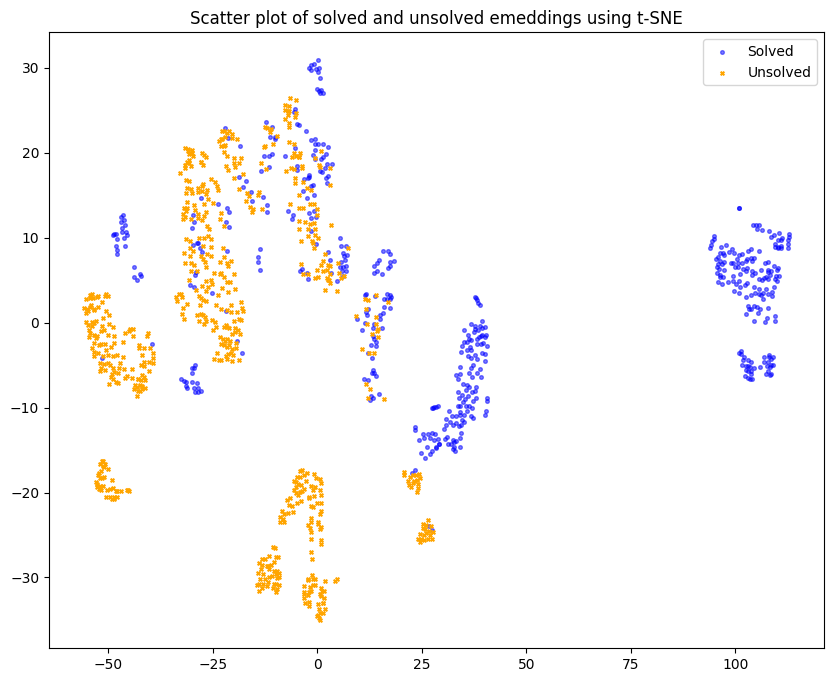
\includegraphics[width=\linewidth]{fig/embeddings_easy_vs_hard.png}
		\caption{Scatter plot of BFS-easy and BFS-hard examples using t-SNE}
		\label{fig:hist_vs_length}
	\end{subfigure}
	\caption{Projection of embeddings to a plane using t-SNE with cosine similarities}\label{fig:embeddings_tsne}
\end{figure}


\fixme{Is one way to interpret this result that the application of  BFS moves takes us far away from the initial presentation, but it still remembers which presentations should be hard vs easy?}
